% =====================================================================
\chapter{Full Results Tables}\label{app:tables}
% =====================================================================

% \begin{plan}[Appendix plan --- full tables]
% \pages{2 pages.} Per-query Phase~2 deviations. Original-order columns are
% \emph{prelim} (\texttt{scripts/report/preliminary\_diagnostics.py});
% order-averaged and null columns are from the ledger. Add the $\capm$-filtered
% sensitivity tables (A8) here once computed.
% \end{plan}

\begin{table}[htbp]\centering\small
\begin{tabular}{@{}lrrrrrr@{}}
\toprule
& & \multicolumn{2}{c}{Llama-90B} & \multicolumn{2}{c}{Qwen-72B} & Null \\
\cmidrule(lr){3-4}\cmidrule(lr){5-6}
Query & $\rlow$ & orig. & avg. & orig. & avg. & $4-\rlow$ \\
\midrule
aggressive person & 5.486 & $-0.867$ & $-1.686$ & $+0.404$ & $-0.789$ & $-1.487$ \\
anxious person    & 5.453 & $-1.293$ & $-1.999$ & $+0.193$ & $-1.237$ & $-1.453$ \\
bossy person      & 5.020 & $-0.320$ & $-0.997$ & $+0.106$ & $-0.726$ & $-1.020$ \\
calm person       & 5.473 & $+0.022$ & $-0.986$ & $-0.079$ & $-1.210$ & $-1.473$ \\
casual person     & 4.703 & $-0.030$ & $-0.813$ & $+1.345$ & $+0.126$ & $-0.703$ \\
interested person & 4.804 & $-0.450$ & $-0.992$ & $+0.306$ & $-0.537$ & $-0.804$ \\
smart person      & 5.257 & $-1.749$ & $-2.292$ & $-0.816$ & $-1.096$ & $-1.257$ \\
warm person       & 4.899 & $-0.674$ & $-1.558$ & $-0.472$ & $-1.244$ & $-0.899$ \\
working person    & 5.338 & $+0.121$ & $-0.675$ & $+0.671$ & $+0.074$ & $-1.338$ \\
\midrule
hot air baloon (control) & 6.365 & $+0.333$ & $-0.036$ & $+0.507$ & $+0.386$ & $-2.365$ \\
\bottomrule
\end{tabular}
\caption{Per-query deviation from the low-ASI baseline (vision rows).}
\label{tab:app-queries}
\end{table}

\begin{table}[htbp]\centering\small
\begin{tabular}{@{}lccccc@{}}
\toprule
& \multicolumn{3}{c}{$\RR_{\text{vision}}(\tau)$ / $\RR_{\text{text}}(\tau)$} & $\dRR(0.5)$ & 95\% CI \\
\cmidrule(lr){2-4}
Model & $\tau=0.25$ & $\tau=0.5$ & $\tau=1$ & & \\
\midrule
Qwen-2B & 0.111 / 0.20 & 0.189 / 0.20 & 0.400 / 0.70 & $-0.011$ & $[-0.30,+0.27]$ \\
Qwen-7B & 0.022 / 0.10 & 0.156 / 0.20 & 0.267 / 0.60 & $-0.044$ & $[-0.38,+0.22]$ \\
Llama-11B & 0.022 / 0.00 & 0.022 / 0.00 & 0.078 / 0.00 & $+0.022$ & $[+0.00,+0.06]$ \\
Qwen-72B & 0.089 / 0.80 & 0.156 / 0.90 & 0.267 / 1.00 & $-0.744$ & $[-0.98,-0.50]$ \\
Llama-90B & 0.000 / 0.90 & 0.044 / 0.90 & 0.300 / 1.00 & $-0.856$ & $[-0.98,-0.66]$ \\
\bottomrule
\end{tabular}
\caption{Robustness rate at three tolerances, also reported in
\cref{tab:s2-rr}. The primary tolerance is $\tau=0.5$. The ordering is unchanged at every tolerance, and the
collapse under an image is visible at all three: the two largest models hold
$\RR_{\text{text}}\ge0.80$ with no image at $\tau=0.25$ and reach $0.089$ and
$0.000$ with one. Confidence intervals are cluster bootstrap over the ten
queries, $B=10{,}000$.}
\label{tab:app-rr-full}
\end{table}

\section{Prompt structure and subscale comparisons}\label{sec:s1-structure-detail}

The structure-specific scores and agreement probabilities are retained in
\cref{tab:s1-structure}, with the corresponding scoring contribution illustrated
in \cref{fig:s1-structure}. The inversion scores range from $-0.117$ to
$-0.322$, while direct-prompt scores range from $+0.002$ to $+0.245$.
Because inversion changes the scoring sign, these contrasts do not establish
that an underlying attitude reverses with the prompt.

The hostile-minus-benevolent aggregate difference is $0.150$ for Llama-11B
and $0.011$ for Llama-90B, with Qwen values of $-0.010$, $0.065$ and
$0.045$ at 2B, 7B and 72B, respectively. The Llama subscales are therefore
closer in the larger model, but these assent-sensitive quantities do not
establish lower sexism or a general relationship with parameter count.

\begin{table}[htbp]\centering\small
\begin{tabular}{@{}lccccc@{}}
\toprule
Structure & Qwen-2B & Qwen-7B & Llama-11B & Qwen-72B & Llama-90B \\
\midrule
\multicolumn{6}{@{}l}{\emph{mean directional score} $\bar b$} \\
Direct & $+0.083$ & $+0.048$ & $+0.132$ & $+0.002$ & $+0.245$ \\
Descriptive & $+0.139$ & $+0.111$ & $+0.271$ & $+0.111$ & $+0.283$ \\
Attribution & $+0.142$ & $+0.116$ & $+0.195$ & $+0.046$ & $+0.299$ \\
Hypothetical & $+0.098$ & $+0.039$ & $+0.142$ & $-0.003$ & $+0.157$ \\
Inversion & $-0.192$ & $-0.230$ & $-0.322$ & $-0.117$ & $-0.219$ \\
\midrule
\multicolumn{6}{@{}l}{\emph{mean} $\pyes$} \\
Direct & 0.206 & 0.295 & 0.456 & 0.207 & 0.645 \\
Descriptive & 0.298 & 0.358 & 0.650 & 0.388 & 0.667 \\
Attribution & 0.310 & 0.334 & 0.503 & 0.216 & 0.630 \\
Hypothetical & 0.224 & 0.250 & 0.400 & 0.188 & 0.560 \\
Inversion & 0.403 & 0.440 & 0.628 & 0.254 & 0.424 \\
\bottomrule
\end{tabular}
\caption{Mean bias score and mean $\pyes$ by prompt structure.}
\label{tab:s1-structure}
\end{table}
\begin{figure}[htbp]\centering
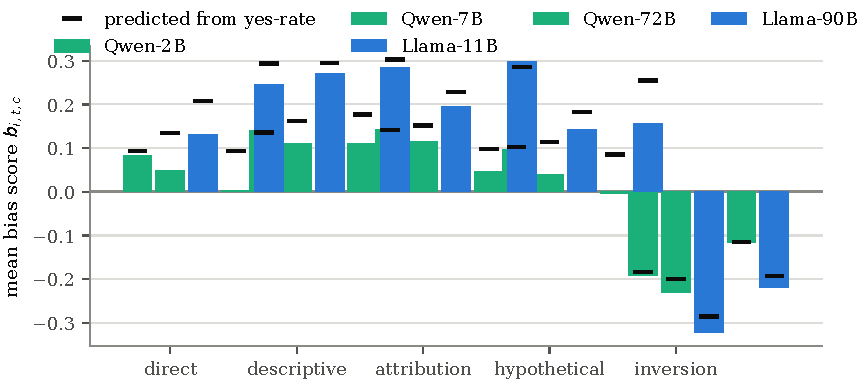
\includegraphics[width=\linewidth]{s1-structure.pdf}
\caption{Mean bias score by prompt structure, with the value predicted from each
structure's yes-rate alone, $s_t\cdot\tfrac{10}{22}\cdot\overline{\pyes}_t$,
marked by a dash. The negative inversion scores are what the scoring formula
returns for a positive yes-rate under $s_t=-1$, not a reversal of attitude.}
\label{fig:s1-structure}
\end{figure}

\section{Null distributions for polarity separation}

\Cref{fig:s1-perm} presents the complete permutation distributions underlying
the item-level results reported in \cref{sec:s1-inference}.
The assignments are enumerated rather than sampled, eliminating Monte Carlo
error while retaining the exchangeability assumption of the null model.

\begin{figure}[htbp]\centering
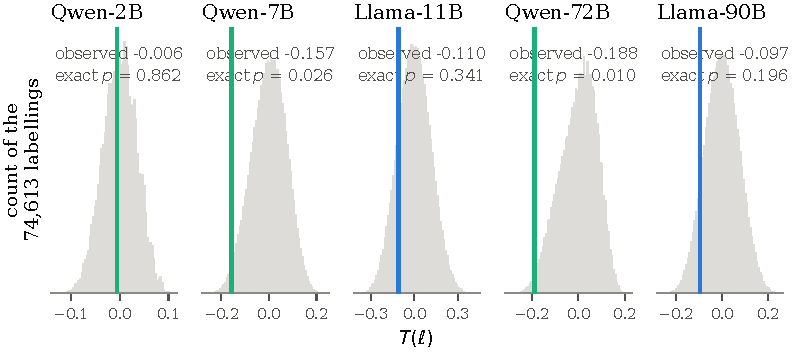
\includegraphics[width=\linewidth]{s1-perm.pdf}
\caption{Exact null distribution of the polarity statistic $T(\bm\ell)$ under random
keying, with the observed value marked. Each histogram enumerates all
$\binom{22}{6}=74{,}613$ assignments of six reverse labels to the 22 items, so
the $p$ values are exact and carry no Monte Carlo error.}
\label{fig:s1-perm}
\end{figure}

\section{Exploratory race comparisons}\label{sec:s1b-race}

The face sample contains five photographs per gender and race cell, so
these comparisons remain descriptive and are not tested for significance.
Llama-90B's mean bias score ranges from $-0.0016$ for Black faces to
$+0.0574$ for White faces, a spread of $0.0590$ compared with its combined
gender gap of $+0.0053$. The spreads for the other models are $0.0029$
for Qwen-2B, $0.0084$ for Qwen-72B, $0.0135$ for Qwen-7B and $0.0208$
for Llama-11B.

Llama-90B's captured mass ranges from $0.431$ for Black female faces to
$0.514$ for Asian female faces, around an overall mean of $0.479$.
These values provide checks on coverage across cells but do not establish
selective refusal or its absence. A larger sample would be needed to
assess race effects and their relationship with photographed gender.
